% !TEX root=/home/tavant/these/manuscript/src/manuscript.tex

\section{Full dielectric model }
  \label{sec-fulldiel}
  
  We have observed the effects of the electron emission and the electrostatic boundary condition separately in \cref{sec-diel_layer,sec-see}, respectively.  
  In \Cref{sec-see}, we observed three regimes depending on the emission rate.
  At high emissivity, the sheath is space-charge limited, resulting in an inverse sheath.
  At low emissivity, we obtain the standard sheath model with electron emission.
  The transition between the regimes passes by a oscillating regime.
  
  In \Cref{sec-diel_layer} we observed that when there is no emission, the dielectric boundary condition for the potential does not change the simulation results.
  In this section, we investigate the interaction between the two characteristics of the dielectric walls, especially with a high emission rate.
  More precisely, regime {\bf II} is the most interesting, as it features a complex behavior.
  Hence, we use $\crover=45\,\volt$ to study the impact of the dielectric layer combined with the electron emission.
  
  The dielectric layer thickness is $L_{\rm Diel} = 3\,\milli\meter$, and the relative permittivity of the dielectric is $\epsilon_R=25$.
  The dimensions of the plasma domain is not modified between the case with and without the dielectric layer.
  Instead, it is the width between the grounded electrodes that is increased.
  
  \subsection{Impact of the dielectric boundary condition on the mobility with electron emission}
    
    \Cref{fig-temporal_mu} shows the temporal evolution of the electron mobility measured in the simulation $\mobpic$ for both cases, with and without the dielectric layer.
    We can see that the two variables are quite similar, with similar mean values and oscillation.
    Interestingly, the beginning of the simulations, up to $t=3\,\micro\second$, are almost identical.
    After this, the values are no more in phase, but follow a similar behavior.
    
    \begin{figure}[hbt]
      \centering
      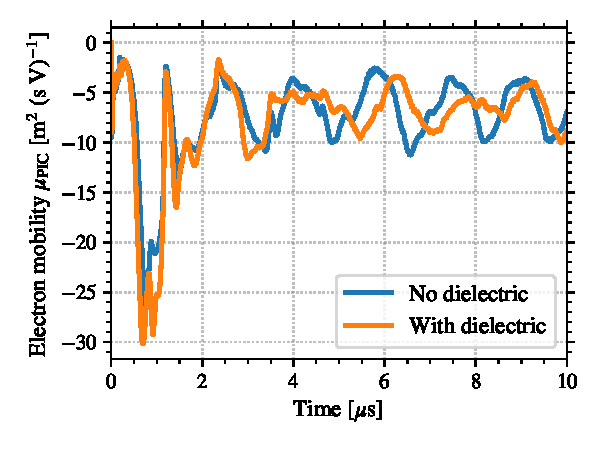
\includegraphics[width=\defaultwidth]{dielectron_yesSEE_mobility}
      \caption{Temporal evolution of the axial electron mobility measured in the \acs{PIC} simulation with and without the dielectric layer between the plasma and the grounded electrodes. The crossover energy is $\crover=45\,\volt$, the length of the dielectric layer is $L_{\rm Diel}=3\milli\meter$ and its relative permittivity is $\epsilon_R = 25$.  }
      \label{fig-temporal_mu} 
    \end{figure}
    
    Hence, we conclude that results concerning the electron mobility obtained in \cref{sec-see} without the dielectric layer modeled will apply as well with the dielectric electrostatic boundary condition.
    In the next section, we analyze the plasma-wall interaction is more details.
    
  \subsection{Plasma-wall interaction}

  \begin{figure}[hbt]
    \centering
    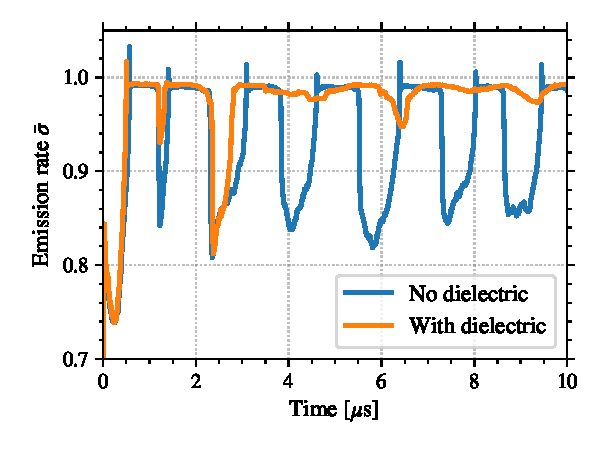
\includegraphics[width=\defaultwidth]{dielectron_yesSEE_SEErate}
    \caption{Temporal evolution of the mean electron emission rate $\ratepic$ averaged over all the wall surface with and without the dielectric layer modeled, for the same value $\crover=45\,\volt$.}
    \label{fig-rso_diel}
  \end{figure}
  
  \Cref{fig-rso_diel} compares the temporal evolution of the mean electron emission rate $\ratepic$ for the same parameter $\crover=45\,\volt$, with and without the dielectric wall modeled.
  As previously, the dielectric width is $3\,\milli\meter$, and the electrodes are now $2.6\,\centi\meter$ apart (the geometry of the plasma domain is kept constant).
  As previously with the electron mobility, the two case present the same result at the beginning, up to $t=2\,\micro\second$.
  After that, the value of $\ratepic$ in the case with the dielectric layer oscillates lightly close to the critical value $\ratecr$, in contrast to the case without the dielectric layer that shows large variations.
  As \cref{fig-rso_diel} shows the values average over all of the wall, it can hide spatial variations.
  Hence the next figures present localized values.
  
  \Cref{fig-seediel_Er_time} shows the temporal evolution of the radial electric field in the sheath at the center of the azimuthal direction ($\theta=0.25 \,\centi\meter$) for {(\bf a)} the case with grounded wall, and {(\bf b)} the case with dielectric layers.
  Only the two millimeters close to the walls are shown, as the radial electric field in the plasma bulk is close to zero.
  On both cases, we can see the sharp transitions between the sheath with high electric field (low $\ratepic$) and the \ac{SCL} regime with low electric field, for which $\ratepic \simeq \ratecr$.
  Hence, in contrast to what could be understood from the mean \ac{SEE} rate in \cref{fig-rso_diel}, the case with dielectric layer do present the \ac{RSO} oscillations.
  For the case without the dielectric layers (\cref{fig-seediel_Er_time}.{\bf a}) the transitions between the left of the right wall are synchronous, as there appears simultaneously on the two walls.
  
  \begin{figure}[hbt]
    \centering
    \begin{tabular}{@{} c c}
      \subfigure{Er_2dcut_noDiel_RSO}{\Large a}{10,5} & 
      \subfigure{Er_2dcut_Diel_RSO}{\Large b}{10,5}
    \end{tabular}
    \caption{Temporal evolution of the radial electric field over 2$\,\milli\meter$ from the wall at the center of the azimuthal direction ($\theta=0.25 \,\centi\meter$) for {(\bf a)} the case with grounded wall, and {(\bf b)} the case with dielectric layers. }
    \label{fig-seediel_Er_time}
  \end{figure}

  On the other hand, the case with dielectric layers presents asynchronous transitions starting from $t=2\,\micro\second$ and later.
  This is why the \ac{RSO} oscillations could not be seen on $\ratepic$ in \cref{fig-rso_diel}.
  In addition, it seems that the left wall remains longer in the \ac{SCL} regime compared to the right wall.
  \Cref{fig-seediel_Er_time_theta} shows the temporal evolution of the radial electric field at the right wall and along the azimuthal direction for {(\bf a)} the case with grounded wall, and {(\bf b)} the case with dielectric layers.
  We see that for the case without the dielectric layer modeled, the sheath changes from the standard regime to the \ac{SCL} regime simultaneously along the radial direction.
  However, in the case with the dielectric layer, the sheath does not necessarily present the same regime at the same time along the azimuthal direction.
  This difference is due to the azimuthal electric field, that must be zero along the wall when the dielectric layer is not modeled, whereas it is not constrained with the dielectric layer modeled.
  
  \begin{figure}[!hbt]
    \centering
    \begin{tabular}{@{} c c}
      \subfigure{ch3_noDiel_2dcut_azimuthal}{\Large a}{10,5} & 
      \subfigure{ch3_Diel_2dcut_azimuthal}{\Large b}{10,5}
    \end{tabular}
    \caption{Temporal evolution of the radial electric field at the wall along the azimuthal direction for {(\bf a)} the case with grounded wall, and {(\bf b)} the case with dielectric layers. }
    \label{fig-seediel_Er_time_theta}
  \end{figure}
  
  
  To finish with, we show in \Cref{fig-surfacecharge} the temporal evolution of the electric field measured in the simulation at the wall and the electric field that corresponds to the surface charge $\frac{\sigma}{\epsilon_0}$ at the center of the azimuthal direction ($\theta=0.25 \,\centi\meter$).
  While the surface charge follows slightly the transitions between the \ac{SCL} and the usual sheath regime, it is significantly different from the measured electric field.
  Especially during the \ac{SCL} regime, where the surface charge shows large oscillations that is not observed on the radial electric field.
  
  \begin{figure}[!hbt]
    \centering
    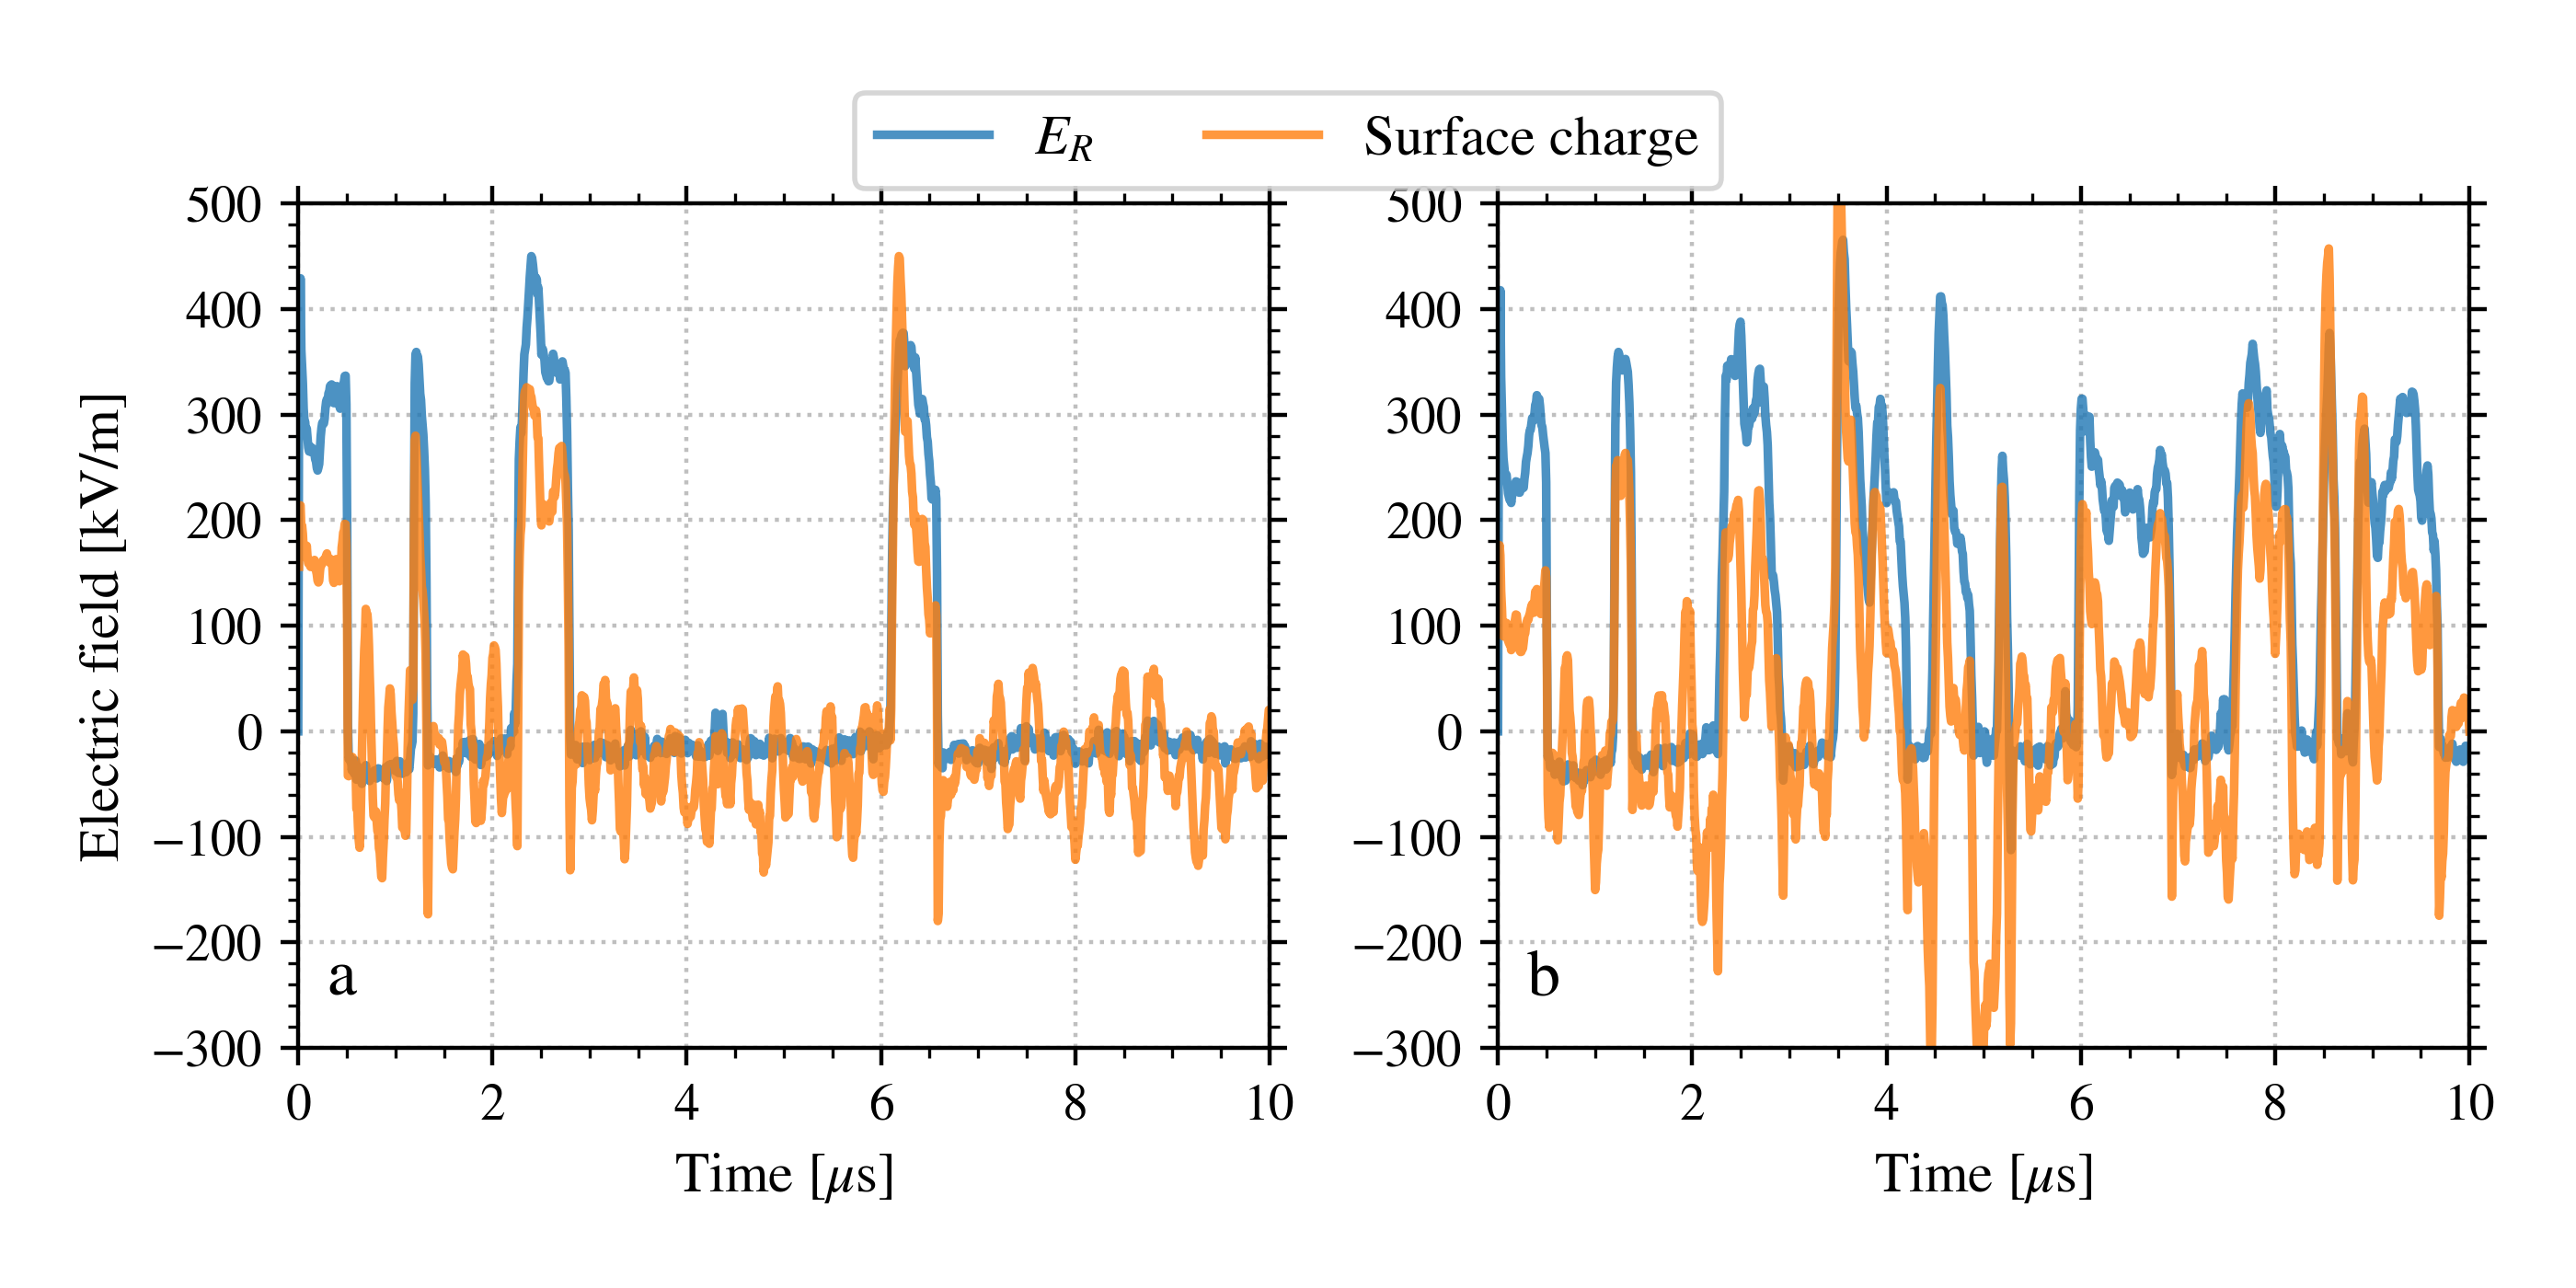
\includegraphics[width=0.9\textwidth]{ch3_Er_vs_sigma_diel}
    \caption{Temporal evolution of (blue) the electric field at the wall and (orange) the electric field that corresponds to the surface charge $\frac{\sigma}{\epsilon_0}$ at the center of the azimuthal direction ($\theta=0.25 \,\centi\meter$) for ({\bf a}) the left wall and ({\bf b}) the right wall. The sign of the electric field is positive toward the wall.}
    \label{fig-surfacecharge}
  \end{figure}
  
  To summarized, we have compared in this section the results of the regime {\bf II} ($\crover=45\,\volt$) with and without the dielectric layer modeled.
  While the transitions between the \ac{SCL} (regime {\bf I} and the usual sheath (regime {\bf III}) is seen in both cases, when the dielectric layer is modeled the transitions are not synchronous between the two walls and along the azimuthal direction.
  Consequently, the sharp transitions of the averaged \ac{SEE} rate $\ratepic$ observed in regime {\bf II} without the dielectric layer is not observed.
  This could explain why this regime has not yet been observed experimentally, as it is very localized.
  Lastly, we observed that the surface charge does not presents the same evolution than the radial electric field at the wall, especially during the \ac{SCL} regime.
  This means that using the Neumann boundary condition to model the dielectric layer will certainly return different results.
  
  